\newpage
\section{Visionneuse Openseadragon}
\label{sec:seadragon}
OpenSeadragon est une visionneuse d’image haute résolution et customisable, open source adaptée aux périphériques desktop et mobiles, ce qui convient à notre projet. Nous utiliserons la version 2.1.0 d'Openseadragon. Openseadragon est un pluggin implémenté en Javascript. La visionneuse sera insérée dans la page HTML de consultation de documents à travers un script comme l'illustre la figure \ref{seadragon}. Pour notre projet nous allons utiliser les fonctionnalités d'Openseadragon suivantes : 
\begin{itemize}
	\item l'affichage de l'image associée au document : Opensedragon prend en charge plusieurs formatq d'images. Dans notre cas, les images de presse anciennes étant très grandes, l'utilisation du format d'image simple(JPG,PNG,...) rend la visionneuse moins performantes. Nous allons donc utiliser un outils, PHP Deep Zoom Tools qui permet d'avoir des images tuilées au format .dzi(Deep Zoom Image), beaucoup plus performantes avec Openseadragon.
	\item les boutons de zoom/dezoom 
	\item les boutons de naviguation, rotation
	\item les overlays : utiles pour délimiter les articles, ou rajouter des tags par exemple. Ici nous rajouterons à Openseadragon le pluggin (javascript égalment) SVG-overlay qui permet de réaliser ces overlays
	  \begin{figure}[H]
        \centering
        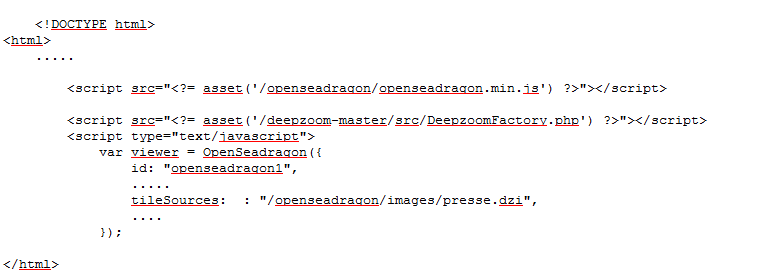
\includegraphics[width=\textwidth]{figure/osd.png}
            \caption{Architecture globale de la plateforme}
            \label{seadragon}
    \end{figure}
	
	





